\documentclass[border=5pt]{standalone}
\usepackage[utf8]{inputenc}
\usepackage{amsmath}
\usepackage{amssymb}

\usepackage{tikz}
\usetikzlibrary{shapes.geometric, arrows}

\tikzstyle{startstop} = [rectangle, rounded corners, minimum width=3cm, minimum height=1cm,text centered, draw=black, fill=red!30]
\tikzstyle{io} = [trapezium, trapezium left angle=70, trapezium right angle=110, minimum width=3cm, minimum height=1cm, text centered, draw=black, fill=blue!30]
\tikzstyle{process} = [rectangle, minimum width=3cm, minimum height=1cm, text centered, draw=black, fill=orange!30]
\tikzstyle{decision} = [diamond, minimum width=3cm, minimum height=1cm, text centered, draw=black, fill=green!30]
\tikzstyle{arrow} = [thick,->,>=stealth, rounded corners]
\tikzstyle{fdot} = [circle, minimum width=4pt, fill]
\tikzstyle{line} = [thick,>=stealth]

\begin{document}

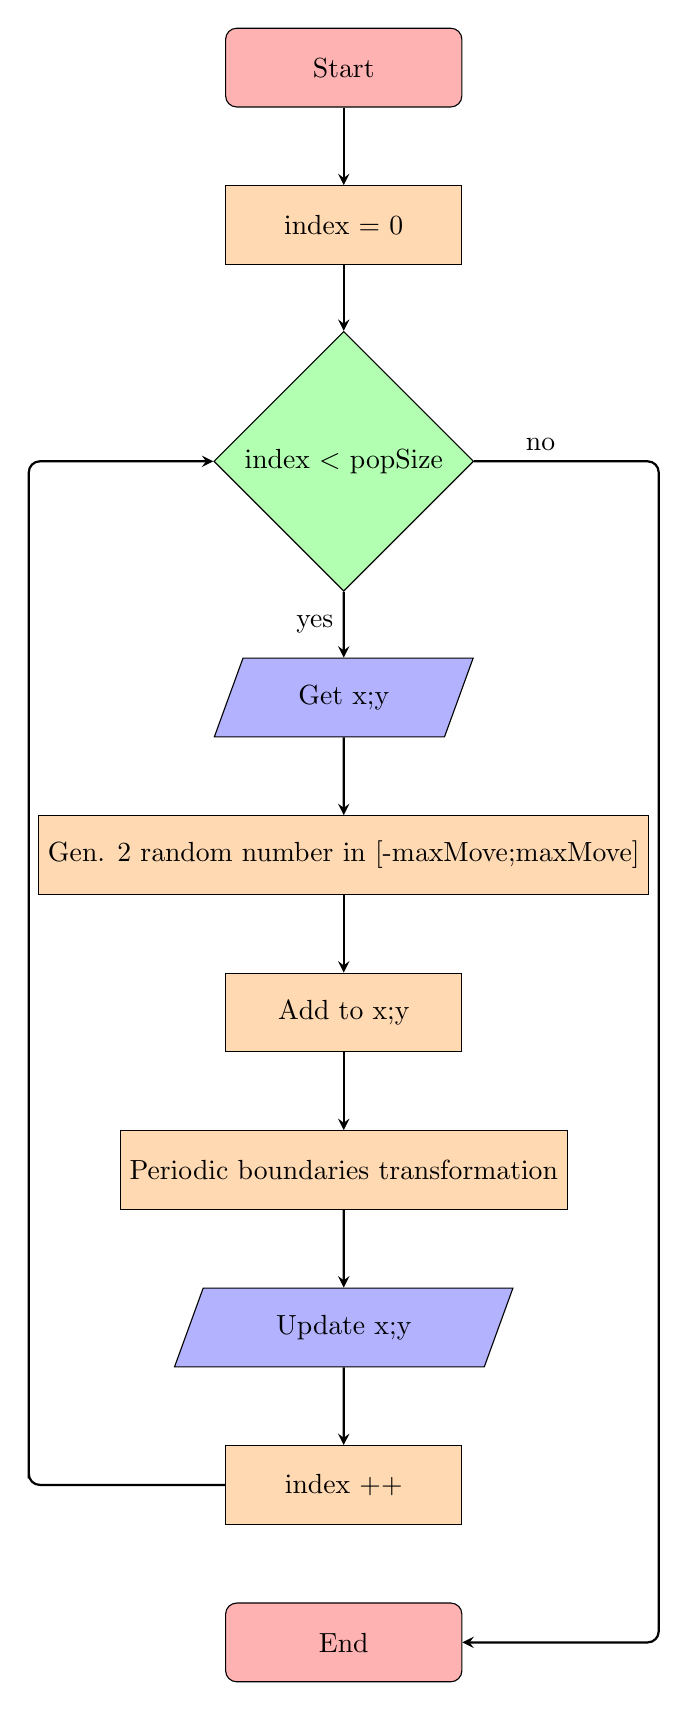
\begin{tikzpicture}[node distance=3cm]

\node (start) [startstop] {Start};
\node (pro1) [process, below of=start, yshift=1cm] {index = 0};
\node (dec1) [decision, below of=pro1] {index $<$ popSize};
\node (in) [io, below of=dec1] {Get x;y};
\node (pro2) [process, below of=in, yshift=1cm] {Gen. 2 random number in [-maxMove;maxMove]};
\node (pro3) [process, below of=pro2, yshift=1cm] {Add to x;y};
\node (pro4) [process, below of=pro3, yshift=1cm] {Periodic boundaries transformation};
\node (out) [io, below of=pro4, yshift=1cm] {Update x;y};
\node (pro5) [process, below of=out, yshift=1cm] {index ++};
\node (stop) [startstop, below of=pro5, yshift=1cm] {End};

\draw [arrow] (start) -- (pro1);
\draw [arrow] (pro1) -- (dec1);
\draw [arrow] (dec1) -- node[anchor=east] {yes} (in);
\draw [arrow] (pro5) -| + (-4,0) |- (dec1);
\draw [arrow] (dec1) -| node[anchor=south, xshift=-1.5cm] {no} + (4,-0.5) |- (stop);
\draw [arrow] (in) -- (pro2);
\draw [arrow] (pro2) -- (pro3);
\draw [arrow] (pro3) -- (pro4);
\draw [arrow] (pro4) -- (out);
\draw [arrow] (out) -- (pro5);

\end{tikzpicture}

\end{document}